\documentclass[aspectratio=169,10pt]{beamer}
% build with   lualatex -shell-escape
% see makefile

% fallback search path for ../theme/ when TEXINPUTS is not set (e.g. texmaker
% quick build); the makefile's TEXINPUTS takes precedence, so no conflict
\makeatletter
\providecommand*{\input@path}{}
\edef\input@path{\input@path{../theme/}{../theme/moloch/}}
\makeatother

\usepackage{icl26}
\deftranslation[to=English]{Theorem}{theorem}
\deftranslation[to=English]{Definition}{definition}
\deftranslation[to=English]{Definitions}{definitions}
\deftranslation[to=English]{Lemma}{lemma}
\newtheorem{proposition}[theorem]{proposition}
\newtheorem{conjecture}[theorem]{conjecture}

\usepackage{multimedia}

\newcommand{\bb}{\mathbf{b}}
\newcommand{\bg}{\mathbf{g}}
\newcommand{\bn}{\mathbf{n}}
\newcommand{\bq}{\mathbf{q}}
\newcommand{\bu}{\mathbf{u}}
\newcommand{\bv}{\mathbf{v}}
\newcommand{\bx}{\mathbf{x}}

\newcommand{\bU}{\mathbf{U}}

\newcommand{\bzero}{\symbf{0}}

\newcommand{\cK}{{\mathcal{K}}}
\newcommand{\cQ}{{\mathcal{Q}}}
\newcommand{\cV}{{\mathcal{V}}}
\newcommand{\cX}{{\mathcal{X}}}

\newcommand{\CC}{{\mathbb{C}}}
\newcommand{\RR}{{\mathbb{R}}}

\newcommand{\mm}{\mathrm{m}}
\newcommand{\nn}{\mathrm{n}}
\newcommand{\pp}{\mathrm{p}}
\newcommand{\qq}{\mathrm{q}}
\newcommand{\rr}{\mathrm{r}}

\newcommand{\eps}{\epsilon}

\newcommand{\grad}{\nabla}
\newcommand{\Div}{\nabla\cdot}

\newcommand{\rhoi}{\rho_{\text{i}}}

\newcommand{\jump}[1]{[\![#1]\!]}

\newcommand{\lc}{{\text{\large $\circ$}}}

% grey comments on the right
\newcommand{\afcomm}[1]{\ensuremath{\text{\footnotesize \grey{$\leftarrow$ #1}}}}
\newcommand{\pcomm}[1]{\grey{\small (#1)}}
\newcommand{\pfcomm}[1]{\grey{\footnotesize (#1)}}

% source of a picture: tiny grey, at right, underneath
\newcommand{\figcite}[1]{\par\nointerlineskip\vskip0.5mm\hbox to \linewidth{\hss\scriptsize\grey{#1}}}


% author photos, stacked at the far right of a frame; paths are relative to talk4/:
%   \begin{withpeople}{\photo{figs/people/a.jpg}{A.~Name} \photo{../talk2/figs/people/b.jpg}{B.~Name}} ... frame body ... \end{withpeople}
% (optional arg of \photo is the height, for longer stacks)
% use ../talk2/figs/people/generic.png when none was found
\newcommand{\photo}[3][10mm]{\hbox to \linewidth{\hss\includegraphics[height=#1]{#2}}\nointerlineskip\vskip0.2mm\hbox to \linewidth{\hss\tiny #3}\vskip0.6mm}
\newenvironment{withpeople}[1]
  {\def\peoplestack{#1}\begin{columns}[T,onlytextwidth]\begin{column}{0.88\textwidth}}
  {\end{column}\begin{column}{0.11\textwidth}\raggedleft\vspace*{-2mm}\peoplestack\end{column}\end{columns}}


\title{The mathematical problem of glaciation}

\subtitle{and a bit of its numerics}

\author{Ed Bueler}

\institute{University of Alaska Fairbanks}

%\date{Imperial College London \, 2026}
\date{BAS \, 2026}


\begin{document}

\begin{frame}
  \titlepage
  \begin{tikzpicture}[remember picture,overlay]
    \node[anchor=south east,inner sep=5mm] at (current page.south east)
      {
\includegraphics[width=25mm]{figs/uafbw.png}};
  \end{tikzpicture}
\end{frame}

\section{pictures: glaciers and ice sheets}

\begin{frame}{Northern Hemisphere ice sheets come and go}

\begin{center}
\begin{tikzpicture}
  \node[anchor=south west,inner sep=0] (map) {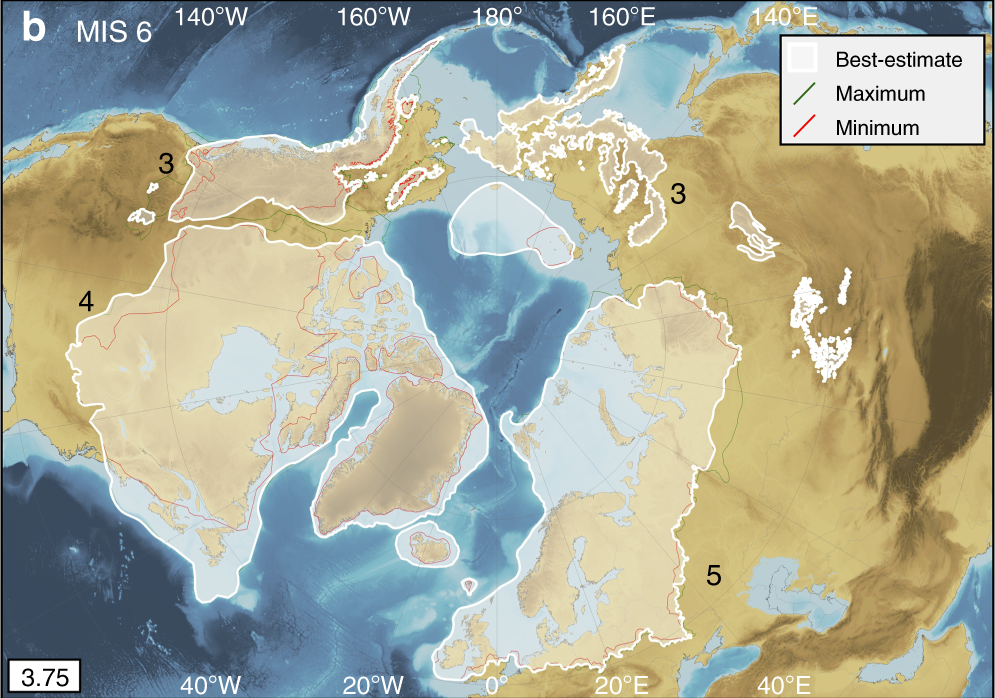
\includegraphics[height=0.76\textheight]{figs/nh-batchelor2019.png}};
  \begin{scope}[x={(map.south east)},y={(map.north west)}]
%    \fill[icAccent] (0.494,0.045) circle (1.8pt);
%    \node[icAccent,font=\footnotesize\bfseries,anchor=west] at (0.57,0.15) (lon) {London};
%    \draw[icAccent,thin] (lon.west) -- (0.494,0.045);
    \fill[icAccent] (0.494,0.047) circle (1.8pt);
    \node[icAccent,font=\footnotesize\bfseries,anchor=west] at (0.57,0.15) (lon) {Cambridge};
    \draw[icAccent,thin] (lon.west) -- (0.494,0.047);
    \fill[icAccent] (0.382,0.762) circle (1.8pt);
    \node[icAccent,font=\footnotesize\bfseries,anchor=west] at (0.45,0.85) (fbk) {Fairbanks};
    \draw[icAccent,thin] (0.45, 0.84) -- (0.382,0.762);
    \fill[icAccent] (0.500,0.503) circle (1.8pt);
    \node[icAccent,font=\footnotesize\bfseries,anchor=west] at (0.57,0.42) (np) {North Pole};
    \draw[icAccent,thin] (np.west) -- (0.500,0.503);
  \end{scope}
\end{tikzpicture}
\end{center}

\vspace{-2mm}
\figcite{best-estimate extent at Marine Isotope Stage 6 ($\sim$140,000 years before present)}

\figcite{Fig.~1b from Batchelor et al (2019), Nature Commun.~10, 3713; added \alert{red} labels}
\end{frame}


\begin{frame}{North American glaciation from 18ka BP to near present}
\centering
\mbox{%
\foreach \n in {1,...,13}{%
  \includegraphics<\n>[height=0.85\textheight,page=\n]{figs/dalton2020-every3.pdf}%
}
% optional: auto-advance in fullscreen mode instead of clicking
%\transduration<1-11>{0.7}
\begin{minipage}{0.3\textwidth}
\grey{\scriptsize from Dalton et al (2020), \par Quaternary Science Reviews 234}
\end{minipage}
}
\end{frame}


\begin{frame}{glaciers are gravity- and climate-driven flows}

\begin{columns}
\begin{column}{0.5\textwidth}
\only<1>{
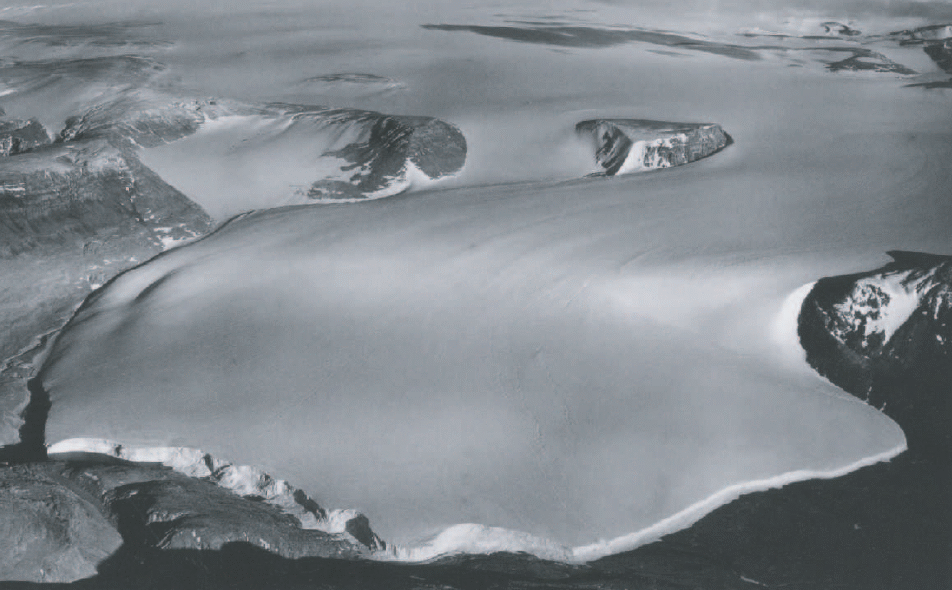
\includegraphics[width=\textwidth]{figs/polaris.png}
\figcite{Polaris Glacier, Greenland; Post \& LaChappelle 2000}
}
\only<2>{
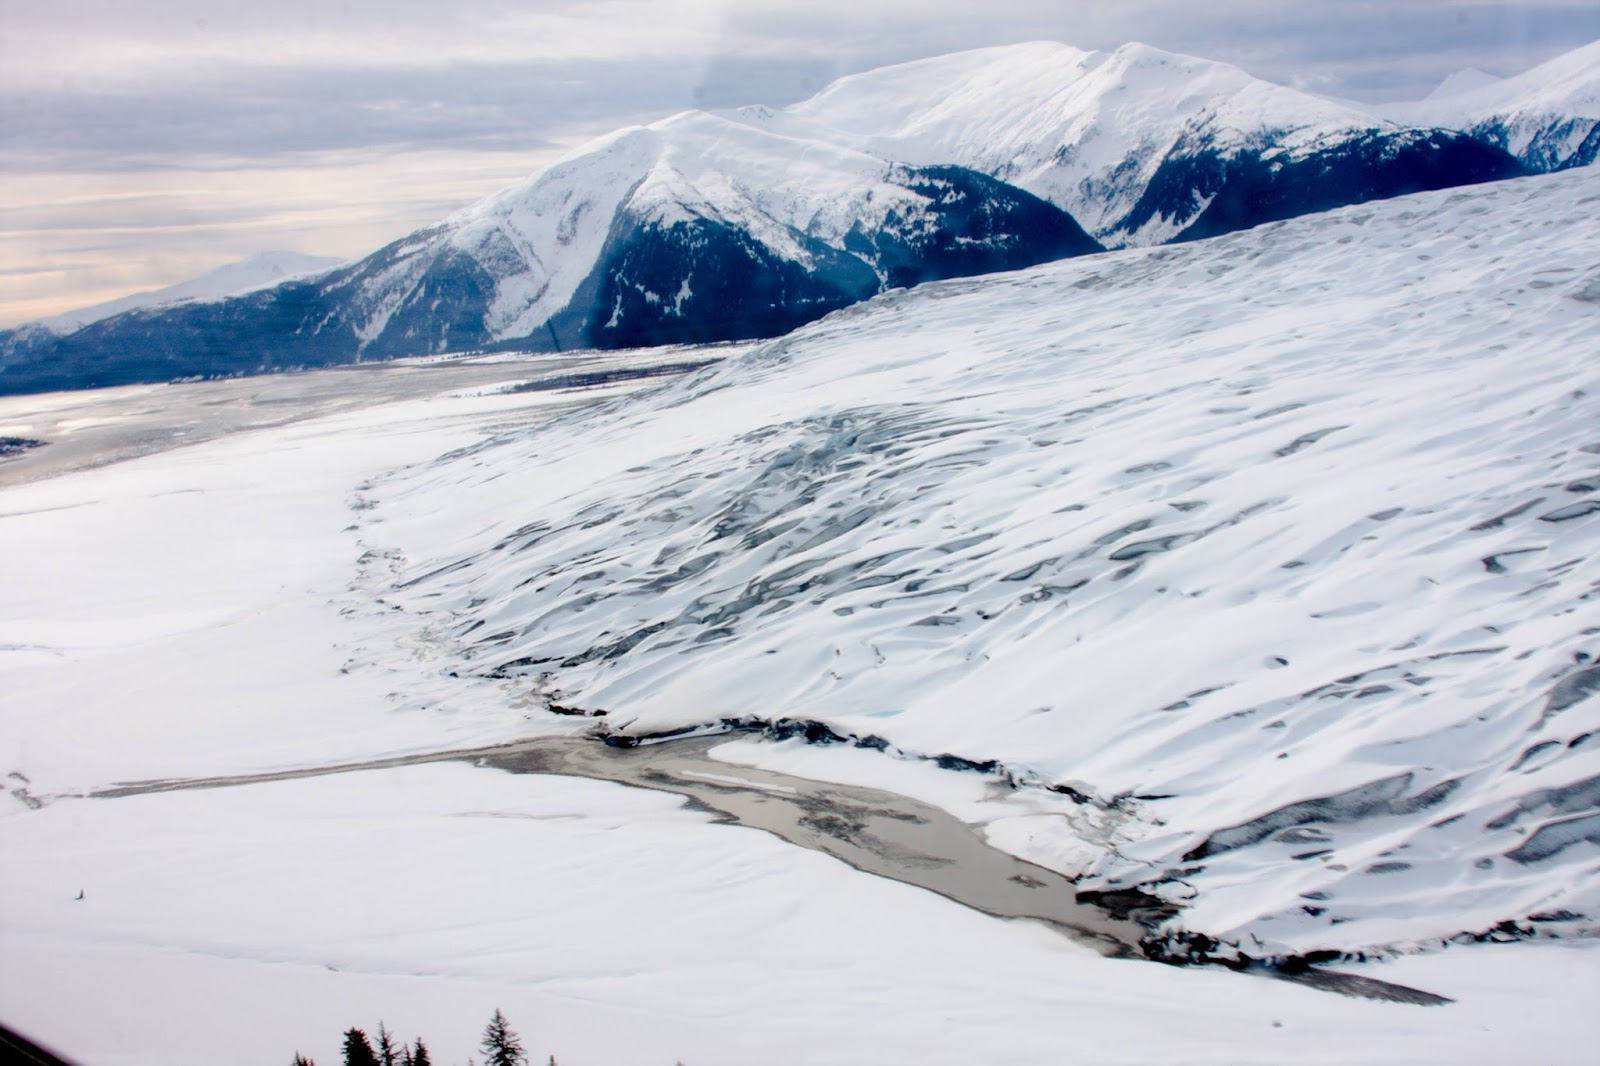
\includegraphics[width=\textwidth]{figs/truffertaku2016.jpg}
\figcite{M.~Truffer photo; Taku Glacier 2016}
}
\end{column}
\begin{column}{0.5\textwidth}
\begin{itemize}
\item a \alert{glacier} is water ice in a very-viscous, gravity-driven flow
    \begin{itemize}
    \item[$\circ$] formed from compressed snow
    \end{itemize}
\item an \alert{ice sheet} is just a big glacier
    \begin{itemize}
    \item[$\circ$] continental scale
    \item[$\circ$] \emph{sea ice} is something quite different
    \end{itemize}
\item \alert{glaciation} means the glacier-covered, time-dependent 2D domain
\item<2> the \alert{glacier margin} is the free boundary of glaciation
    \begin{itemize}
    \item[$\circ$] location determined by combined effects of climate, bed topography, boundary stresses, and ice flow
    \item[$\circ$] steeper surface slopes near margins
    \item[$\circ$] non-fluid features (fractures and crevasses) often dominate margins at small scale
    \end{itemize}
\end{itemize}
\end{column}
\end{columns}
\end{frame}


\begin{frame}{qualitative observations about present-day ice sheets}

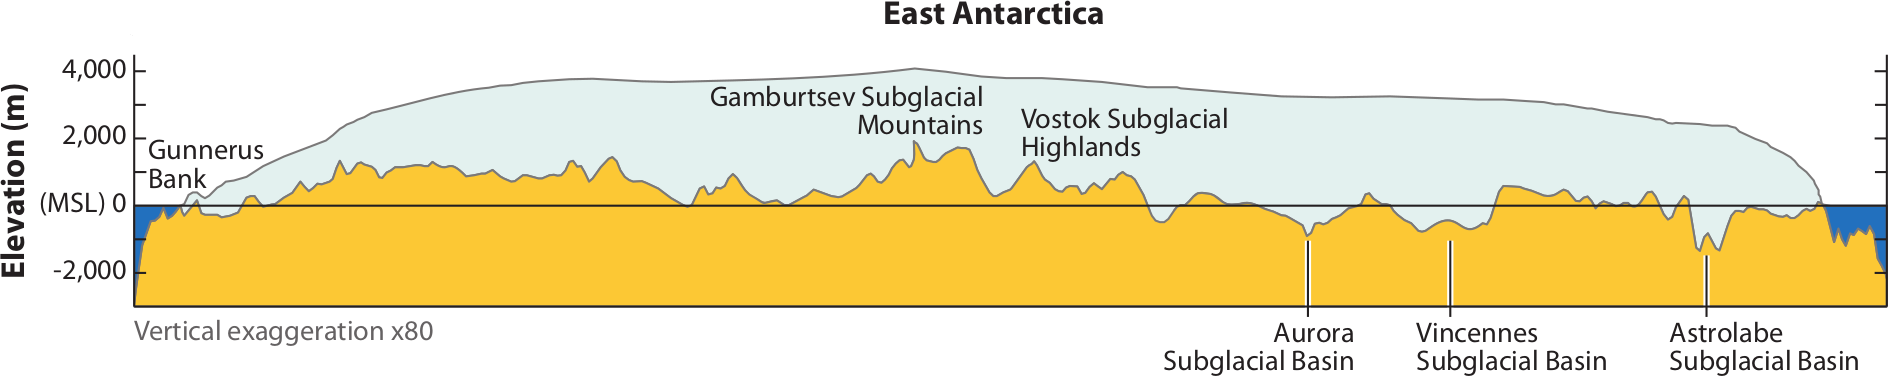
\includegraphics[width=\textwidth]{figs/ant-schoofhewitt2013.png}

\medskip
\figcite{cross-section of East Antarctica, with \alert{80$\times$ vertical exaggeration}}

\figcite{Schoof \& Hewitt (2013), Annu.~Rev.~Fluid Mech.~45, 217--239}

\medskip
\begin{itemize}
\item there are two present-day ice sheets: Antarctica (big!), Greenland (medium)

\item very thin (in aspect-ratio sense)
\item smooth surface, often above a rough bed
\item steeper surface slopes near margins
\end{itemize}
\end{frame}


\begin{frame}{qualitative observations about present-day ice sheets}

\begin{columns}
\begin{column}{0.6\textwidth}
\hfill 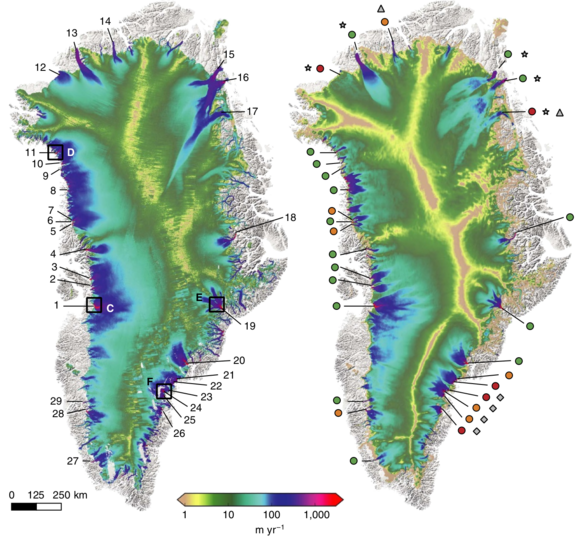
\includegraphics[width=0.93\textwidth]{figs/gis-aschwanden2016.png}
\end{column}
\begin{column}{0.4\textwidth}
\vspace{20mm}

\begin{itemize}
\item large velocity contrasts
\item fast flow concentrated in narrow outlets near boundary
\item nearly-fractal boundaries
\end{itemize}

\vspace{20mm}
\grey{\scriptsize Greenland surface speed

\alert{left: observed}, \, right: modeled

Aschwanden et al (2016), Nature Commun.~7, 10524

}
\end{column}
\end{columns}
\end{frame}


\begin{frame}{outline}
  \tableofcontents
\end{frame}


\begin{frame}[standout]
\begin{itemize}
\item I welcome questions at any time!
\item they are a \emph{good} use of time
\end{itemize}
\end{frame}


\section{mathematical models of glaciation}

\begin{frame}{notation for evolving glaciers}

\hfill\includegraphics<1>[width=0.54\textwidth]{figs/notation1.pdf}%
\includegraphics<2>[width=0.54\textwidth]{figs/notation2.pdf}

\begin{overprint}
\onslide<1>
\vspace{-8mm}

\begin{itemize}
\item fixed land domain \alert{$\Omega\subset\RR^2$}
    \begin{itemize}
    \item[$\lc$] $x = (x_1,x_2) \in \Omega$
    \end{itemize}
\item \alert{surface mass balance} $a(t,x)$ \grey{[m$\,$a$^{-1}$;\, the climate as seen by the glacier]} \hfill \grey{$\leftarrow$ data}
    \begin{itemize}
    \item[$\lc$] $a>0$ is accumulation of snow
    \item[$\lc$] $a<0$ is ablation by melt
    \item[$\lc$] assuming: $a$ is defined everywhere in $\Omega$, \emph{even where there is no ice}
    \end{itemize}
\item \alert{bed elevation} $b(x)$ \grey{[m]} \hfill \grey{$\leftarrow$ data}
    \begin{itemize}
    \item[$\lc$] defined everywhere in $\Omega$
    \end{itemize}
\end{itemize}
\onslide<2>
\begin{itemize}
\vspace{2mm}

\item \alert{surface elevation} $s(t,x)$ \grey{[m]} \hfill \grey{$\leftarrow$ solution}
    \begin{itemize}
    \item[$\lc$] equivalent geometry variable: \alert{thickness} $H(t,x)=s(t,x)-b(x)$
    \item[$\lc$] required:\, $\alert{s(t,x)\ge b(x)} \, \iff \, H(t,x)\ge 0$
    \end{itemize}
\item \alert{ice domain} $\displaystyle \Lambda(t) = \left\{(x,z) \,:\, b(x) < z < s(t,x)\right\} \subset \RR^3$  \hfill \grey{$\leftarrow$ solution}
    \begin{itemize}
    \item[$\lc$] this 3D set is an output, \emph{not data}
    \item[$\lc$] \alert{glaciation} is \, $\Lambda(t)^\perp = \left\{x \,:\, b(x) < s(t,x)\right\} \subset \Omega$, also an output
    \end{itemize}
\end{itemize}
\end{overprint}
\end{frame}


\begin{frame}{how does the glacier surface move?}

\hfill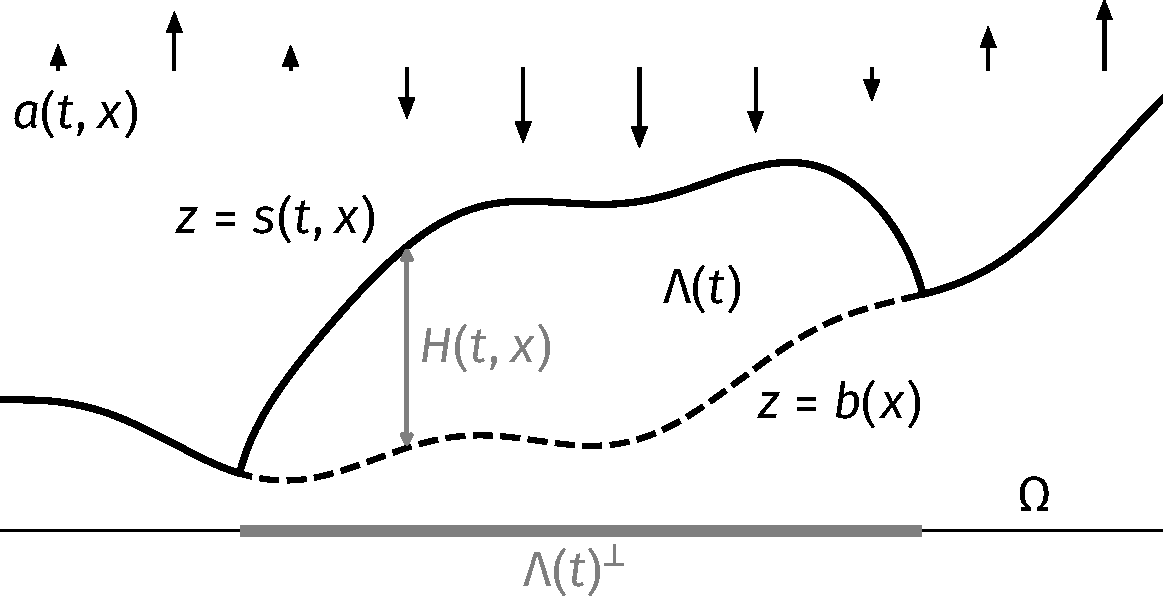
\includegraphics[width=0.35\textwidth]{figs/notation2.pdf}

\begin{itemize}
\item \alert{surface kinematical equation}:
\begin{equation*}
\frac{\partial s}{\partial t} + \bu|_s \cdot \bn_s = a
\end{equation*}

    \begin{itemize}
    \item[$\lc$] $\bu|_s$ is the surface trace of 3D ice velocity
    \item[$\lc$] $\bn_s = \left<-\tfrac{\partial s}{\partial x_1}, -\tfrac{\partial s}{\partial x_1}, 1\right>$ is the upward surface normal vector
    \item[$\lc$] derive via e.g.~apply pillbox mass-conservation argument
    \end{itemize}

\medskip
\item this equation applies at the (non-material) surface $z=s(t,x)$ \alert{only if  $s(t,x) > b(x)$},
\item so it \alert{cannot}, by itself, describe the evolution of glaciation
\end{itemize}
\end{frame}


\begin{frame}{surface elevation view: advection with inequality constraint}

\hfill 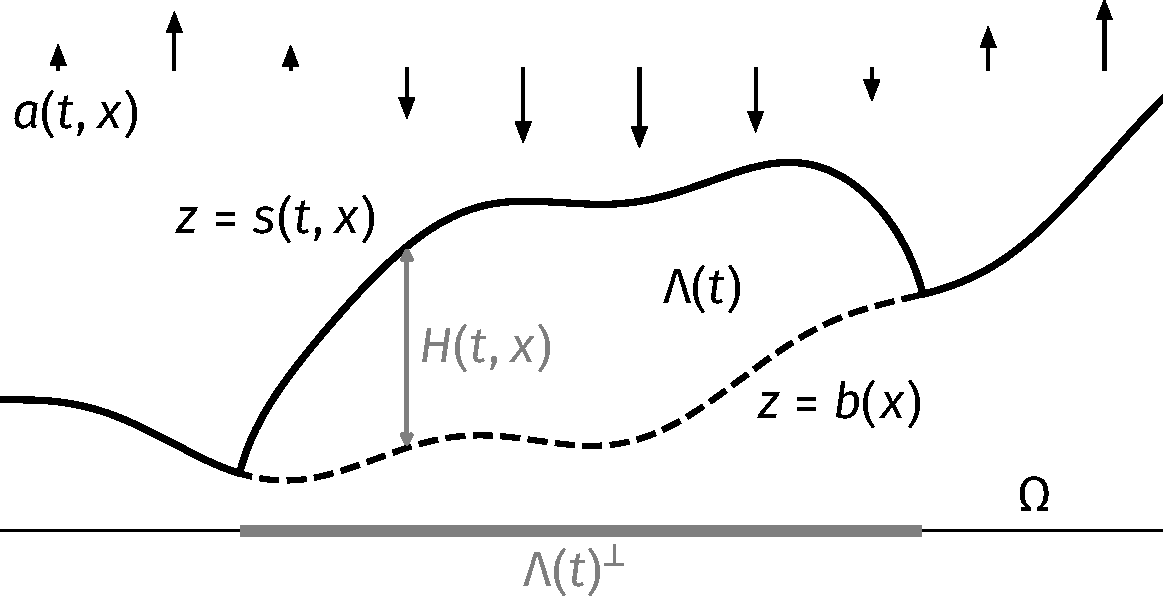
\includegraphics[width=0.35\textwidth]{figs/notation2.pdf}

\vspace{-5mm}
\begin{itemize}
\item Q: how does the glacier and the glaciation \alert{evolve}?
    \begin{itemize}
    \item[$\lc$] for the moment, ignoring the stress balance in $\Lambda(t)$
    \end{itemize}

\pause
\item A: via a \alert{nonlinear complementarity problem} (NCP) on $[0,T]\times\Omega$:
\begin{align*}
s - b &\ge 0 \\
\frac{\partial s}{\partial t} + \bu|_s \cdot \bn_s - a &\ge 0 \\
(s-b) \left(\frac{\partial s}{\partial t} + \bu|_s \cdot \bn_s - a\right) &= 0
\end{align*}

    \begin{itemize}
    \item[$\lc$] assuming: \,\alert{$s=b$} and \alert{$\bu|_s$ is extended by zero} over ice-free land

    \end{itemize}
\end{itemize}

\grey{
\only<2>{\strut \phantom{foo}}
\only<3>{\strut where $s>b$: \, $\frac{\partial s}{\partial t} + \bu|_s \cdot \bn_s = a$}
\only<4>{\strut at ice-free locations $s=b$: \, $\partial s/\partial t=0$ and $\bu|_s=\bzero$ therefore $a\le 0$, ablation}
}
\end{frame}


\begin{frame}{thickness view: conservation with inequality constraint}

\hfill 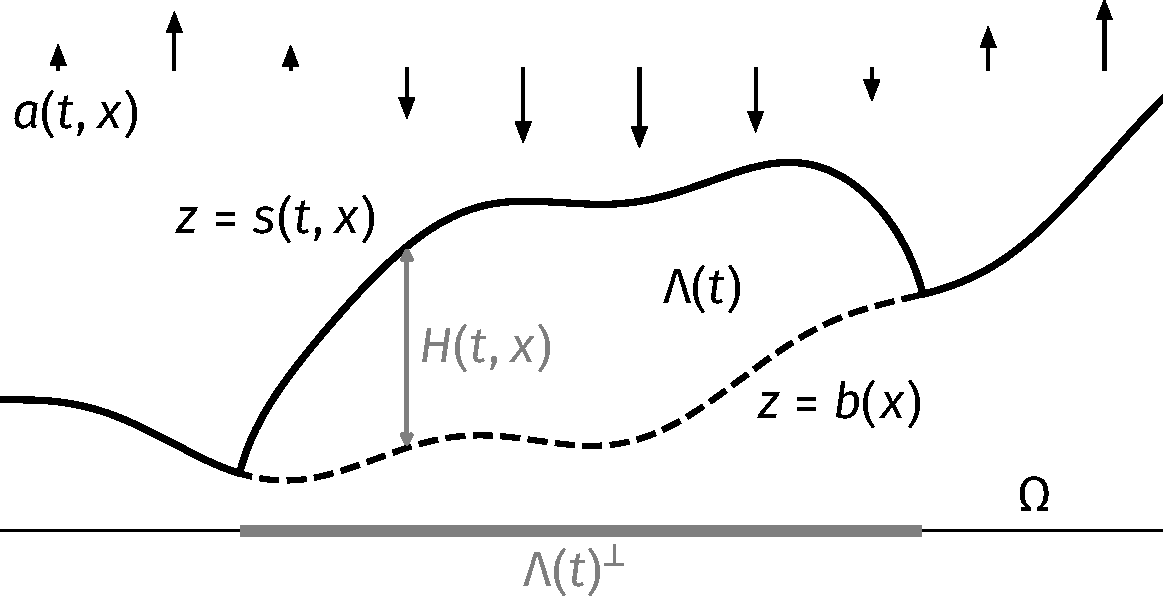
\includegraphics[width=0.35\textwidth]{figs/notation2.pdf}

\vspace{-15mm}
\begin{itemize}
\item another view, equally valid, using thickness:

\quad $H(t,x)=s(t,x)-b(x)$
\item $\bU=$ (horizontal ice velocity in $\Lambda(t)$)
\item define the \alert{ice flux}:
$$\alert{\bq(t,x)=\int_{b(x)}^{s(t,x)} \bU(t,x,z)\,dz} \hspace{30mm}$$
\item again an NCP:

\vspace{-5mm}
{\small
\begin{align*}
H &\ge 0 \\
\frac{\partial H}{\partial t} + \Div\bq - a &\ge 0 \\
H\left(\frac{\partial H}{\partial t} + \Div\bq - a\right) &= 0
\end{align*}
}

    \begin{itemize}
    \item[$\lc$] \alert{where ice is present}, $H > 0$, \alert{mass is conserved}: \,$\frac{\partial H}{\partial t} + \Div\bq - a = 0$
    \item[$\lc$] at ice-free locations ($H=0$, $\partial H/\partial t = 0$, $\bq=\bzero$) we have $a\le 0$, ablation
    \end{itemize}
\end{itemize}
\end{frame}


\begin{frame}{equivalence: weak surface motion equals weak flux divergence}

\begin{itemize}
\item recall equivalent equations, applying where $s>b$ and $H > 0$:
   $$\frac{\partial s}{\partial t} + \bu|_s \cdot \bn_s = a \qquad \leftrightarrow \qquad \frac{\partial H}{\partial t} + \Div\bq = a$$

    \begin{itemize}
    \item[$\lc$] let's call $\bu|_s \cdot \bn_s$ the \alert{surface motion}
    \end{itemize}
\end{itemize}

\begin{lemma}
If ice is incompressible $\Div \bu=0$, and if $\bu|_b\cdot \hat\bn = 0$, then for any test function $\omega(x)$ on $\Omega$:

\hspace{30mm} $\displaystyle \alert{\int_\Omega (\bu|_s\cdot \bn_s)\, \omega \,dx = \int_\Omega \bq \cdot \grad \omega\,dx}$.
\end{lemma}

\pause
{\footnotesize
\noindent \textbf{proof.} \, Extend to $\Lambda(t)\subset \RR^3$:\, $\omega(x)=\tilde\omega(x,z)$.  Recall $\bn_s = \left<-\grad s,1\right>$.  Then
\begin{align*}
\int_\Omega (\bu|_s\cdot \bn_s)\, \omega\,dx &= \int_{\partial\Lambda(t)} \tilde\omega\,\bu\cdot\hat\bn\,ds && \afcomm{only top contributes;\, \alert{$\bn_s\,dx=\hat\bn\,ds$}} \\
&= \int_{\Lambda(t)} \Div\left(\tilde\omega\,\bu\right)\,dx\,dz = \int_{\Lambda(t)} \bu\cdot\grad\tilde\omega\,dx\,dz && \afcomm{div theorem;\, \alert{incompressibility}} \\
&= \int_\Omega \bq \cdot\grad\omega\,dx && \afcomm{$\tilde\omega$ indep of $z$;\, def of $\bq$} \hspace{15mm} \hfill \qed
\end{align*}
}
\end{frame}


\begin{frame}{why prefer surface elevation?}

\centering
\mbox{%
\hspace{20mm}
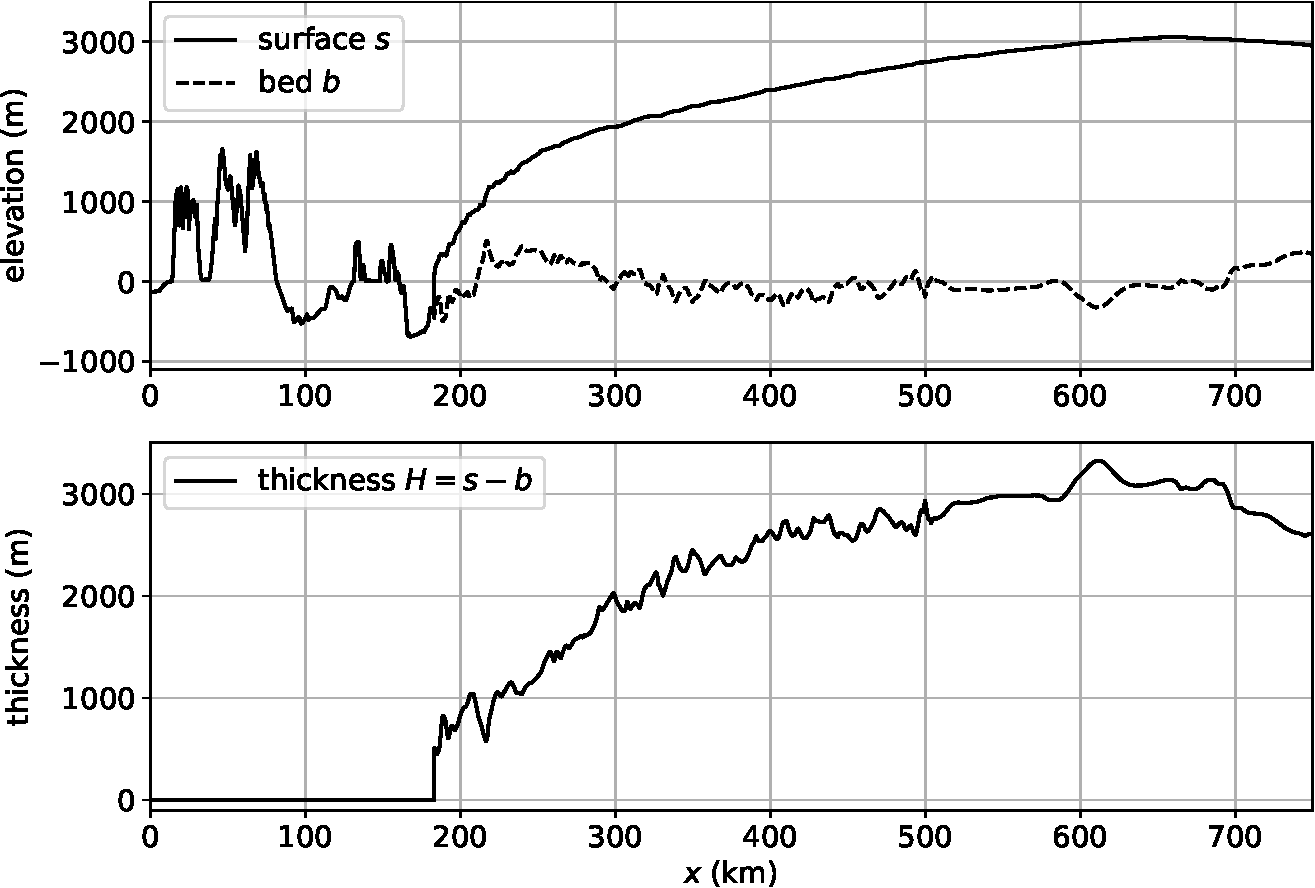
\includegraphics[height=0.65\textheight]{figs/giscross.pdf} \,
\begin{minipage}{0.3\textwidth}
\vspace{-5mm}

\grey{\scriptsize Greenland cross-section at $70^\circ$N

data from Morlighem et al.~2017}
\end{minipage}
}

\medskip
\begin{itemize}
\item gravity-driven ice \alert{flow causes the surface $s(t,x)$ to become smoother}
\item meanwhile $H(t,x)=s(t,x)-b(x)$ inherits the (spatial) low regularity of the bed
\end{itemize}
\end{frame}


\begin{frame}{translation: \, glacier language $\leftrightarrow$ optimization language}

\begin{columns}
\begin{column}{0.63\textwidth}
\begin{definition}
An inequality constraint ``$f(x)\ge c$'' is \alert{active} on $\{x\,:\,f(x)=c\}$ and \alert{inactive} otherwise, on $\{x\,:\,f(x)>c\}$.
\end{definition}
\end{column}
\begin{column}{0.37\textwidth}
\hfill \includegraphics<1->[width=\textwidth]{figs/notation2.pdf}
\end{column}
\end{columns}

\bigskip
\begin{itemize}
\item the inequality constraint: \, $s\ge b \iff H\ge 0$

\bigskip
\item for map-plane subsets of $\Omega$, at $t$:

\begin{center}
\begin{tabular}{rcl|c}
glaciology     &                   & optimization  & subset \\ \hline
glaciation     & $\leftrightarrow$ & inactive set  & $\Lambda(t)^\perp${\Large \strut} \\
ice-free area  & $\leftrightarrow$ & active set    & \,\,$\Omega \setminus \Lambda(t)^\perp${\large \strut} \\
glacier margin & $\leftrightarrow$ & free boundary & \,\, $\Omega \cap \partial\Lambda(t)^\perp${\large \strut}
\end{tabular}
\end{center}
\end{itemize}
\end{frame}


\newcommand{\stokesblock}[1]{%
\begin{align*}
-\Div\left(2\nu(D\bu)D\bu\right)+\grad p &= \rhoi\bg && \text{in $\Lambda$} \qquad\qquad\quad \grey{\text{stress balance}} \\
\Div\bu &= 0                                         && \text{in $\Lambda$} \qquad\qquad\quad \grey{\text{incompressible}} \\
\left(2\nu(D\bu)D\bu-pI\right) \hat\bn &= \bzero && \text{on $\Gamma_s\subset\partial \Lambda$ \qquad \grey{stress free}} \\
\bu &= \bzero && \text{on $\Gamma_b\subset\partial \Lambda$ \qquad \grey{#1}}
\end{align*}
}


\begin{frame}{momentum conservation: Stokes}

\begin{itemize}
\item let $\alert{\pp} = 1 + 1/\nn \alert{\approx 4/3}$, where $\nn\approx 3$ is \alert{Glen's exponent} for ice rheology
\item $D\bu = 0.5 (\grad \bu + \grad \bu^\top)$ is the \alert{strain rate}
\item fix $t$ and consider the ice domain $\Lambda=\Lambda(t)=\{(x,z):b<z<s\}$
\item for the \alert{effective viscosity} $\nu(D\bu)=\nu_0 |D\bu|^{\pp-2}$, \hfill \afcomm{$\nu_0>0$ constant, e.g.~isothermal}
\end{itemize}

\vspace{-4mm}
{\small
\stokesblock{\alert{non-sliding} for simplicity}
}

\pause
\vspace{-1mm}
\begin{block}{fixed-domain Stokes well-posedness \grey{(Jouvet \& Rappaz 2011)}}
If $\Lambda$ is a bounded Lipschitz domain then there is a unique $(\bu,p)\in W^{1,\pp}(\Lambda;\RR^3)\times L^{\pp'}(\Lambda)$ solving the above \alert{$\pp$-Stokes problem}.
\end{block}

\begin{itemize}
\item also, a surface trace bound applies:\,$\int_{\Gamma_s}\big|\bu|_s\big|^\pp \le C$ \hfill  \pfcomm{B 2026}
\end{itemize}
\end{frame}


\begin{frame}{we want a glacier \underline{evolution} model}

\begin{itemize}
\item the Stokes block:
{\footnotesize
\stokesblock{non-sliding}
}
\item this has no time derivative, so this is \alert{not an evolution model} by itself
    \begin{itemize}
    \item[$\lc$] the domain $\Lambda(t)$ evolves; it is not fixed in reality
    \item[$\lc$] both surface $s(t,x)$ and domain $\Lambda(t)$ are parts of model solution
    \end{itemize}

\pause
\item evolution model: \alert{couple} Stokes to the \alert{surface kinematical NCP}
$$s - b \ge 0, \qquad
\frac{\partial s}{\partial t} + \bu|_s \cdot \bn_s - a \ge 0, \qquad
(s-b) \left(\frac{\partial s}{\partial t} + \bu|_s \cdot \bn_s - a\right) = 0$$

    \begin{itemize}
    \item[$\lc$] evolving state variables: \,\alert{$s(t,x), \, \bu(t,x,z), \, p(t,x,z)$}
    \end{itemize}
\end{itemize}
\end{frame}


\begin{frame}{the canonical glacier evolution model}

\begin{columns}
\begin{column}{0.555\textwidth}
\begin{block}{surface-Stokes evolution model}
\vspace{-4mm}

{\small
\begin{align*}
s - b &\ge 0 && \text{on $\Omega$} \\
\frac{\partial s}{\partial t} + \bu|_s \cdot \bn_s - a &\ge 0 && \text{on $\Omega$} \\
(s-b) \left(\frac{\partial s}{\partial t} + \bu|_s \cdot \bn_s - a\right) &= 0  && \text{on $\Omega$} \\
-\Div\left(2\nu(D\bu)D\bu\right)+\grad p &= \rhoi\bg && \text{in $\Lambda(t)$} \\
\Div\bu &= 0                                         && \text{in $\Lambda(t)$} \\
\left(2\nu(D\bu)D\bu-pI\right) \hat\bn &= \bzero && \text{on $\Gamma_s(t)\subset \partial\Lambda(t)$} \\
\bu &= \bzero && \text{on $\Gamma_b(t)\subset \partial\Lambda(t)$}
\end{align*}
}
\end{block}
\end{column}
\begin{column}{0.4\textwidth}
\includegraphics[width=1.05\textwidth]{figs/notation3.pdf}

\vfill
\end{column}
\end{columns}

\medskip
\begin{itemize}
\small
\item key definition and coupling:\, $\displaystyle \alert{\Lambda(t) = \left\{(x,z)\,:\,b(x) < z < s(t,x)\right\}}$

\pause
\item the Stokes block acts as an \alert{algebraic constraint} in the coupled dynamical system
\item glacier evolution is a \alert{differential-algebraic system with inequality constraints}
\end{itemize}
\end{frame}


\AtBeginSection[]
{
  \begin{frame}{outline}
  \tableofcontents[currentsection]
  \end{frame}
}


\section{shallow ice approximation is somewhat well-posed}

\begin{frame}{well-posed math problems}

\begin{definition}[Hadamard]
a mathematical problem is \alert{well-posed} if the solution
\begin{enumerate}
\item exists
\item is unique
\item changes continuously as the data (inputs) change
\end{enumerate}
\end{definition}

\pause
\small
\begin{block}{Example: finite-dimensional linear systems}
Given invertible $A$ and vector $\bb$ (of compatible sizes).  Solving $A\bx = \bb$ for $\bx$ is well-posed because
\begin{enumerate}
\item exists: $\bx = A^{-1}\bb$
\item unique: if $A\bx_1=\bb$ and $A\bx_2=\bb$ then $A(\bx_1-\bx_2)=\bzero$ so $\bx_1=\bx_2$
\item continuous in the data $\bb$: if $A\bx_1=\bb_1$ and $A\bx_2=\bb_2$ then

\quad $\|\bx_1-\bx_2\| = \|A^{-1}\bb_1 - A^{-1}\bb_2\| \le \|A^{-1}\| \|\bb_1 - \bb_2\|$
\end{enumerate}
\end{block}
\end{frame}


\begin{frame}{shallow ice approximation (SIA)}

\begin{itemize}
\item first try, historically-speaking:\, the lubrication approximation
    \begin{itemize}
    \item[$\lc$] \alert{shallow ice approximation} evolution model \hfill \pfcomm{Fowler, Larson, Hutter, Halfar 1980s}
    \item[$\lc$] scales: $[L]$ horizontal extent, $[H]$ thickness
    \item[$\lc$] small aspect-ratio limit $\eps=[H]/[L]\to 0$
    \end{itemize}

\pause
\item in limit $\eps\to 0$, the flux $\bq = \int_b^s \bU\,dz$ resolves to a \alert{local differential operator} on $s$:
    $$\hspace{35mm} \bq = -\underbrace{\gamma_0 \, (s-b)^{\nn+2} |\grad s|^{\nn-1}}_{\text{diffusivity } D}\, \grad s \hspace{20mm} \text{\afcomm{$\gamma_0>0$ constant}}$$

    \begin{itemize}
    \item[$\lc$] \alert{ice flows downhill} in this model since $D>0$ \hfill \pfcomm{down $\grad s$; not necessarily down $\grad H$}
    \end{itemize}

\pause
\item thus $s(t,x)$ solves a degenerate, \alert{doubly-nonlinear} PDE where $s>b$:
    $$\frac{\partial s}{\partial t} - \Div\left(\gamma_0 (s-b)^{\nn+2} |\grad s|^{\nn-1}\grad s\right) = a$$

    \begin{itemize}
    \item[$\lc$] in the SIA, $s$ solves a \alert{diffusion}
    \end{itemize}
\end{itemize}
\end{frame}


\begin{frame}{flat bed: well-posedness for 1D time-dependent SIA}

\begin{itemize}
\item for $b=0$, SIA evolution is a clean NCP:
    $$s\ge 0, \qquad F(s)\ge 0, \qquad s F(s) = 0 \hspace{40mm}$$

\vspace{-8mm}
\hfill \grey{\scriptsize $\displaystyle \left[F(s) = \frac{\partial s}{\partial t} - \Div\left(\gamma_0 (s-b)^{\nn+2} |\grad s|^{\nn-1}\grad s\right) - a\right]$}
\end{itemize}

\medskip
\begin{theorem}[Calvo, D\'iaz, Durany, Schiavi, V\'azquez 2002]
Suppose $\Omega\subset\RR^1$, bounded data $a(t,x)$, and $b=0$.  For $\mm=2(\nn+1)/\nn \approx 8/3$, there is a unique bounded weak solution $s(t,x) \ge 0$, where \alert{$s^\mm \in L^\qq(0,T;W_0^{1,\qq}(\Omega))$ } for $\alert{\qq}=\nn+1\alert{\approx 4}$.
\end{theorem}

{\small
\noindent \textbf{proof idea.} Use Raviart (1970) power transformation $\alert{w=s^\mm}$ on doubly-nonlinear diffusion.  Converts surface motion into \alert{$\qq$-Laplacian} form:\, $\displaystyle s^{\nn+2} |\grad s|^{\nn-1}\grad s \to c |\grad w|^{\qq-2}\grad w$.
}

\pause
\medskip
\begin{itemize}
\item they proved certain qualities: ablation implies retreat, ``waiting'' possible in advance
\item first recognition that \alert{glacier evolution is a (parabolic) obstacle problem}
\item Piersanti \& Temam (2023): also for 2D flat bed, but with extra technical hypotheses
\end{itemize}
\end{frame}


\begin{frame}{general bed: existence for 2D steady SIA}

\begin{itemize}
\item if $\grad b\ne 0$ then Raviart's power transformation $w=(s-b)^\mm=H^\mm$ implies a \alert{solution-dependent ``tilt''} \, $\grad w \to \grad w + c w^{(\qq+1)/(2\qq)} \grad b$ \, inside the diffusion
\end{itemize}

\begin{withpeople}{\vspace{5mm} \photo[13mm]{figs/people/gjouvet.png}{G.~Jouvet}}
\begin{theorem}[Jouvet \& B 2012]
Suppose $\Omega\subset\RR^2$, $\qq>2$, \alert{general bed $b\in W^{1,\qq}(\Omega)$}, and bounded $a(x)$.  There exists a weak thickness solution $H(x)\ge 0$ to the \alert{steady} SIA obstacle problem, with $H^\mm \in W_0^{1,\qq}(\Omega)$.
\end{theorem}
\end{withpeople}

\medskip
{\small
\noindent \textbf{proof ideas.} The weak form is a \alert{variational inequality} (VI).  Use the Raviart power transformation, freeze the nonlinearities to create monotone VI problems, prove nontrivial \emph{a priori} bound on the iterates \pfcomm{Guillaume!}, and apply Schaefer fixed point theorem.
}

\pause
\medskip
\begin{itemize}
\item \alert{uniqueness was left open}
    \begin{itemize}
    \item[$\lc$] except that it holds in the flat bed case
    \end{itemize}
\end{itemize}
\end{frame}


\begin{frame}{general bed with dips: steady-state uniqueness fails where $a=0$}

\centerline{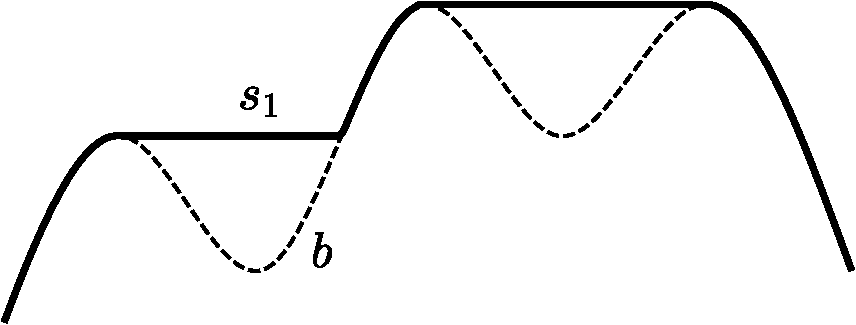
\includegraphics[width=0.33\textwidth]{figs/filled.pdf} \quad 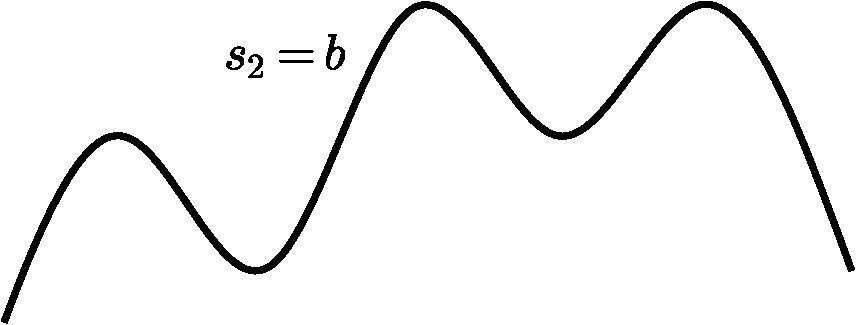
\includegraphics[width=0.33\textwidth]{figs/icefree.pdf}}
\figcite{$s_1$ fills basins with flat ice, $s_2=b$ is ice-free}

\begin{proposition}[B 2026,\footnote{\href{https://arxiv.org/abs/2408.06470}{\emph{Surface elevation errors in FE Stokes models for glacier evolution}, arXiv:2408.06470}} App.~B]
For $\Omega \subset \RR^d$, if $b$ is continuous \alert{with strict local minima}, and then there exist steady climates $a(x)$, with \alert{$a=0$ over the dips}, giving multiple steady solutions for $s(x)$.
\end{proposition}

{\small
\noindent \textbf{proof.} Both $s_1,s_2$ have $\bu|_{s_i}=\bzero$, so both solve NCP when $a=0$ covers the dip:
   $$\hspace{35mm} s-b\ge 0, \quad -\bu|_s\cdot\bn_s\ge 0, \quad (s-b)(\bu|_s\cdot\bn_s)=0. \hspace{35mm} \qed$$
}

\begin{itemize}
\item applies for any stress balance

\pause
\medskip
\item observation: surface motion $\Phi(s) = -\bu|_s\cdot\bn_s$ is \alert{not strictly monotone} as function of $s$
\end{itemize}
\end{frame}


\begin{frame}{SIA well-posedness scorecard}

\begin{center}
\setlength{\tabcolsep}{5pt}
\begin{tabular}{llllll}
 & bed & time & existence & uniqueness \\
\midrule
Calvo et al (2002) & flat (1D) & dependent & yes & yes \\
Piersanti \& Temam (2023) & flat (2D) & dependent & yes$^*$ & -- \\
Jouvet \& B (2012) & general & steady & yes & only flat case \\ \hline
B (2026), App.~B & bumpy & steady & -- & \alert{no}$^\dagger$ when $a\equiv 0$ \\
\midrule
\end{tabular}
\end{center}

\vspace{-2mm}
{\hfill \footnotesize $^*$ several technical conditions}

{\hfill \footnotesize $^\dagger$ applies for any stress balance}

\smallskip
\begin{itemize}
\item open well-posedness problem: time-dependent SIA on a general bed
    \begin{itemize}
    \item[$\lc$] Raviart power transformation may be exhausted, and new ideas needed?
    \end{itemize}

\pause
\medskip
\item but real glaciers and ice sheets are \emph{not} shallow for most scientifically-useful modeling purposes
\item \alert{no such existence results for the canonical surface-Stokes model}
    \begin{itemize}
    \item[$\lc$] this talk is about that, though informed by SIA results
    \end{itemize}
\end{itemize}
\end{frame}


\section{surface-Stokes is nearly coercive}

\begin{frame}{behavior of the surface motion?}

\begin{itemize}
\item for glacier evolution, understanding the ice flow contribution to surface kinematics means understanding the \alert{surface motion} as a nonlinear operator:
    $$s \quad \stackrel{\Phi}{\mapsto} \quad - \bu|_s \cdot \bn_s$$

    \begin{itemize}
    \item[$\lc$] remember this uses Stokes to compute $\bu$
    \end{itemize}
\item more properly it is a weak-form operator:
    $$\hspace{15mm} s \quad \stackrel{\Phi}{\mapsto} \quad -\int_\Omega (\bu|_s \cdot \bn_s)\, \omega \qquad \text{\grey{(for test functions $\omega$)}}$$

    \begin{itemize}
    \item[$\lc$] recall: \, $\displaystyle \int_\Omega (\bu|_s \cdot \bn_s)\, \omega = \int_\Omega \bq(s)\cdot\grad \omega$
    \end{itemize}

\bigskip
\item is $\Phi$ a nice nonlinear operator?  \qquad \only<2>{\grey{what does ``nice'' mean?}}
\end{itemize}
\end{frame}


\begin{frame}{abstract niceness for nonlinear operators}

\begin{itemize}
\item operator of interest: surface motion weak-form \quad $\displaystyle s \, \stackrel{\Phi}{\mapsto} \, -\int_\Omega (\bu|_s \cdot \bn_s)\, \omega$
\end{itemize}

\bigskip
\begin{definitions}
For a Banach space $\cX$, a subset $\cK\subset \cX$, and a nonlinear map $F:\cK\to\cX'$.
\begin{itemize}
\item $F$ is \alert{$\qq$-coercive} if there is $\alpha>0$ so that \alert{$\left(F(v)-F(w)\right)[v-w]\ge\alpha\|v-w\|^\qq$} for all $v,w\in\cK$
\item $F$ is \alert{monotone} if $\left(F(v)-F(w)\right)[v-w] \ge 0$; \, \alert{strictly} if $v\ne w$ implies ``$>$''
\end{itemize}
\end{definitions}

\begin{itemize}
\item $\qq$-coercive \, $\implies$ \, strictly-monotone
\end{itemize}
\end{frame}


\begin{frame}{connecting back to optimization}

\begin{itemize}
\item abstract operator $F:\cK \to \cX'$
\item $F$ is \alert{strictly-monotone} if $\left(F(v)-F(w)\right)[v-w] > 0$ for all $v\ne w$

\bigskip
  \centerline{% general (non-gradient) F(x,y) = A [x y]^T with A = S + R where
% S = [[1, 0.4], [0.4, 0.5]] (same as tikz/gradfield.tex) and R = [[0, -0.8], [0.8, 0]];
% F is strictly-monotone (symmetric part S) but curl F != 0 so F is not grad J
\begin{tikzpicture}[scale=0.65]
  \foreach \x in {-2,-1.5,...,2}
    \foreach \y in {-2,-1.5,...,2} {
      \pgfmathsetmacro{\fx}{\x - 0.4*\y}
      \pgfmathsetmacro{\fy}{1.2*\x + 0.5*\y}
      \draw[-{Stealth[length=1.4mm]}, icAccent] (\x,\y) -- ++({0.15*\fx},{0.15*\fy});
    }
  \fill[icGrey] (0,0) circle (2.5pt) node[right, icGrey, inner sep=1pt, xshift=0.5mm] {\small $F=0$};
  \node at (0,-3.2) {general $F$};
\end{tikzpicture}
 \qquad\qquad \onslide<2>{% F = grad J for strictly-convex J(x,y) = (1/2) [x y] S [x y]^T,
% S = [[1, 0.4], [0.4, 0.5]] (symmetric positive-definite)
% compare: tikz/generalfield.tex has same symmetric part plus a rotation
\begin{tikzpicture}[scale=0.65]
  \begin{scope}
    \clip (-2.6,-2.6) rectangle (2.6,2.6);
    \foreach \c in {0.04,0.15,0.35,0.6,0.9,1.3}
      \draw[icBlue!60, thick] plot[domain=0:360, samples=90, smooth cycle]
        ({sqrt(2*\c/(cos(\x)^2 + 0.8*cos(\x)*sin(\x) + 0.5*sin(\x)^2))*cos(\x)},
         {sqrt(2*\c/(cos(\x)^2 + 0.8*cos(\x)*sin(\x) + 0.5*sin(\x)^2))*sin(\x)});
  \end{scope}
  \foreach \x in {-2,-1.5,...,2}
    \foreach \y in {-2,-1.5,...,2} {
      \pgfmathsetmacro{\fx}{\x + 0.4*\y}
      \pgfmathsetmacro{\fy}{0.4*\x + 0.5*\y}
      \draw[-{Stealth[length=1.4mm]}, icAccent] (\x,\y) -- ++({0.15*\fx},{0.15*\fy});
    }
  \fill[icGrey] (0,0) circle (2.5pt) node[right, icGrey, inner sep=1pt, xshift=0.5mm] {\small $F=0$};
  \node at (0,-3.2) {$F=\grad J$};
\end{tikzpicture}
}}

\pause
\medskip
\item if $F=\grad J$ for a smooth objective $J:\cK\to\RR$ then:

\medskip
\centerline{$F$ strictly-monotone $\iff$ $J$ strictly-convex}
\end{itemize}
\end{frame}


\begin{frame}{coercivity question for weak surface motion}

\vspace{-10mm}

    $$\Phi(s)[\omega] = -\int_\Omega (\bu|_s \cdot \bn_s)\, \omega, \qquad s\in \cK = \{\sigma \,:\,\sigma \ge b\}, \qquad \bu|_s \text{ from Stokes}$$

\medskip
\begin{overprint}
\onslide<1>
\begin{itemize}
\item is $\Phi$ a $\qq$-coercive operator?
\item I have 5 things to say
\end{itemize}
\onslide<2>
\begin{block}{I.~lemma (B, 2026)}
%If $\Lambda(t)$ is a Lipschitz domain then Stokes dynamics will generate a trace $\bu|_s \in L^\pp(\Gamma_s)$.
For any $\qq\ge 2$, \alert{$\Phi$ is a well-defined map} from $s\in \cK \subset \alert{\cX=W^{1,\qq}(\Omega)}$ to $\cX'$.
\end{block}
\onslide<3>
\begin{block}{II.~intuition}
$\Phi$ \alert{should be $2$-coercive} because ice flows downhill.
\end{block}

{\small
\noindent \textbf{argument.}  It is reasonable to believe $\bq(s)\approx -C\grad s$ for $C>0$.  Thus
    $$\left(\Phi(\sigma)-\Phi(s)\right)[\sigma-s] \stackrel{\text{\grey{recall}}}{=} -\int_\Omega \left(\bq(\sigma)-\bq(s)\right)\cdot\grad(\sigma-s) \approx \int_\Omega \left(C\grad(\sigma)-C\grad(s)\right)\cdot\grad(\sigma-s) \ge \tilde C \|\sigma-s\|_{W^{1,2}}^2.$$
}

\medskip
\begin{itemize}
\item the power-law rheology does not appear in this informal reasoning
\end{itemize}
\onslide<4>
\begin{block}{III.~SIA case}
\begin{itemize}
\item In the SIA, $\Phi$ is \alert{not $\qq$-coercive} on $s\in W^{1,\qq}(\Omega)$, for any $\qq$, even in the flat bed case, because the \alert{diffusivity $D$ degenerates at margins}. \hfill {\small \grey{$\leftarrow \quad D = \gamma_0 \, (s-b)^{\nn+2} |\grad s|^{\nn-1}$}}
\item In the SIA flat-bed case $\Phi$ \alert{becomes} $\qq$-coercive, $\qq=\nn+1\approx 4$, \alert{when redefined} by the Raviart transformation.  Now it acts coercively on $w=s^\mm \in W^{1,\qq}(\Omega)$.
\end{itemize}
\end{block}
\onslide<5>
\begin{block}{IV.~counter-example (B, 2026)}
For a bed with local minima, $\Phi$ is \alert{not} strictly-monotone, thus not $\qq$-coercive for any $\qq>0$.
\end{block}

\bigskip
\centerline{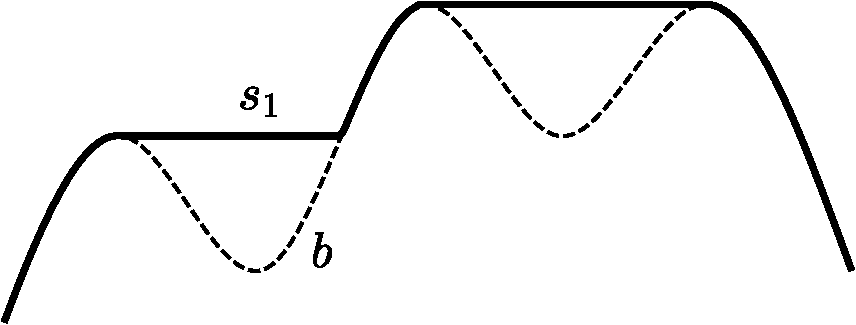
\includegraphics[width=0.33\textwidth]{figs/filled.pdf} \qquad 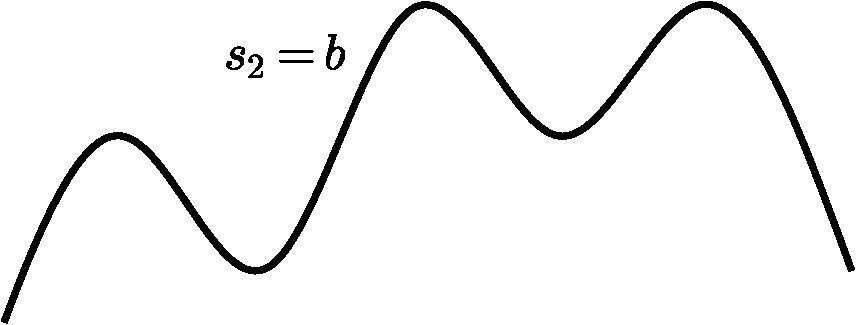
\includegraphics[width=0.33\textwidth]{figs/icefree.pdf}}
\onslide<6>
\begin{block}{V.~speaking for myself}
the coercivity situation is \alert{confusing}
\end{block}
\end{overprint}
\end{frame}


\begin{frame}{numerical coercivity experiment}

\begin{itemize}
\item but the Firedrake 
\includegraphics[width=4mm]{figs/firedrake-small.png} is a good friend

\medskip
\item \alert{run many Stokes simulations} to generate 2000 \alert{random surface pair samples}
    \begin{itemize}
    \item[$\lc$] 1D domain $\Omega$, length 200 km, $h=$ 500 m mesh resolution
    \item[$\lc$] either flat or rough bed, initial ice thickness 1400 m
    \item[$\lc$] 3 different climates, advance/retreat/deglaciation cases
    \end{itemize}

\medskip
\centerline{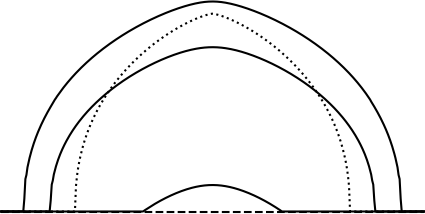
\includegraphics[width=0.32\textwidth]{figs/snapsflat.png} \quad 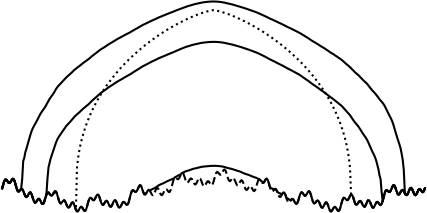
\includegraphics[width=0.32\textwidth]{figs/snapsrough.png}}
\figcite{from B (2026), App.~C}

\item for each pair, \alert{compute the $4$-coercivity ratio} using $W^{1,4}$ norm:
    $$\rho(\sigma,s)=\frac{\left(\Phi(\sigma)-\Phi(s)\right)[\sigma-s]}{\|\sigma-s\|_{W^{1,4}}^4} \hspace{45mm}$$

\vspace{-7mm}
\hfill \grey{\footnotesize $\left(F(v)-F(w)\right)[v-w]\ge\alpha\|v-w\|^\qq \quad \forall v,w\in\cK$}
\end{itemize}
\end{frame}


\begin{frame}{numerical surface-Stokes: nearly coercive?}

\begin{itemize}
\item what do we see?
\end{itemize}

\medskip
\centerline{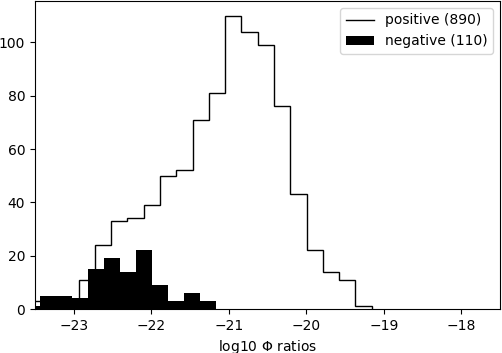
\includegraphics[width=0.44\textwidth]{figs/bflat500mNOREG.png} \quad 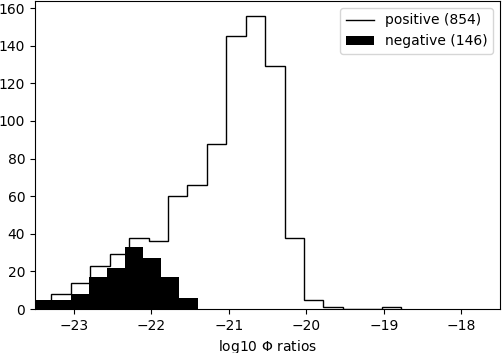
\includegraphics[width=0.44\textwidth]{figs/brough500mNOREG.png}}

\medskip
\figcite{histograms of ratio magnitudes $|\rho(\sigma,s)|$: flat (left) and rough (right) beds}

\medskip
\begin{itemize}
\item more than \alert{10\%} of ratios $\rho(\sigma,s)$ are \alert{negative}, which \alert{violates coercivity}

\pause
\item but magnitudes are much smaller; \alert{Stokes surface motion ``wants'' to be coercive}
\end{itemize}
\end{frame}


\begin{frame}{regularize using SIA-type diffusion}

\begin{itemize}
\item start from weak surface motion with $\bu|_s$ from Stokes: \, $\Phi(s)[\omega] = -\int_\Omega (\bu|_s \cdot \bn_s)\, \omega$
\item choose a fixed thickness $\eta_0>0$, and $0<\eps\ll 1$
\item using SIA formula with $\nn=3$, define
\begin{align*}
\Phi^\eps(s)[\omega] &= (1-\eps)\Phi(s)[\omega] \alert{+\eps\,\gamma_0\eta_0^{5}\int_\Omega|\grad s|^{2}\grad s\cdot\grad\omega}
\end{align*}
\item that is, add a bit of the $4$-Laplacian operator to regularize
\end{itemize}

\pause
\begin{conjecture}[B 2026]
On $\cK = \{\sigma \ge b\} \subset \alert{\cX=W^{1,4}(\Omega)}$, there exist $\eps>0$, $\eta_0>0$, and $\alpha>0$ so that \alert{$\Phi^\eps$ is $4$-coercive}:
    $$\left(\Phi^\eps(\sigma)-\Phi^\eps(s)\right)[\sigma-s]\ge\alpha\|\sigma-s\|_\cX^4 \quad \text{for all } \sigma,s\in\cK.$$
\end{conjecture}
\end{frame}


\begin{frame}{numerical regularized surface-Stokes: credibly coercive}

\centerline{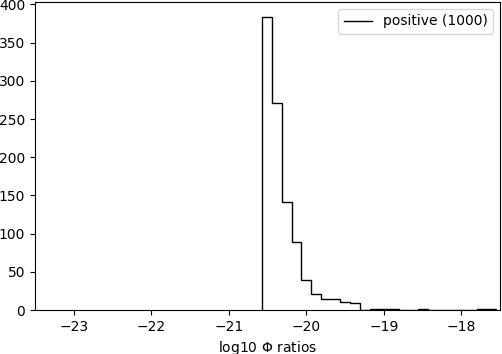
\includegraphics[width=0.44\textwidth]{figs/bflat500mREG.png} \qquad 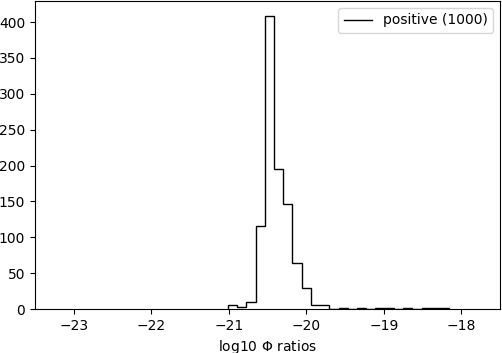
\includegraphics[width=0.44\textwidth]{figs/brough500mREG.png}}

\medskip
\figcite{histograms of regularized ratio magnitudes: flat (left) and rough (right) beds}

\medskip
\begin{itemize}
\item with \alert{$\eps=0.01$} and $\eta_0=500$ m: \, \alert{all ratios are positive}
\item $\alpha=10^{-22}$ is credible in \, ``$\left(\Phi^\eps(\sigma)-\Phi^\eps(s)\right)[\sigma-s]\ge\alpha\|\sigma-s\|_\cX^4$''
\medskip
\item the regularization does not need to do much work
\end{itemize}
\end{frame}


\begin{frame}{what is the regularization doing?}

$$\Phi^\eps(s)[\omega] = -(1-\eps)\int_\Omega (\bu|_s \cdot \bn_s)\, \omega +\eps\,\gamma_0\eta_0^{5}\int_\Omega|\grad s|^{2}\grad s\cdot\grad\omega \qquad \text{with $\bu|_s$ from Stokes}$$

\medskip
\begin{itemize}
\item surface-Stokes evolution only mildly smooths high-frequency surface bumps
\item this $\eps>0$ regularization adds $4$-Laplacian smoothing

\pause
\item now the $s_1$ surface has lower ``energy'' than $s_2$:

\bigskip
\centerline{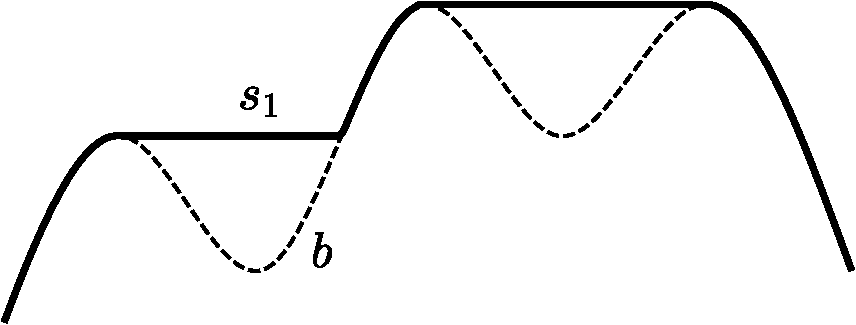
\includegraphics[width=0.26\textwidth]{figs/filled.pdf} \qquad 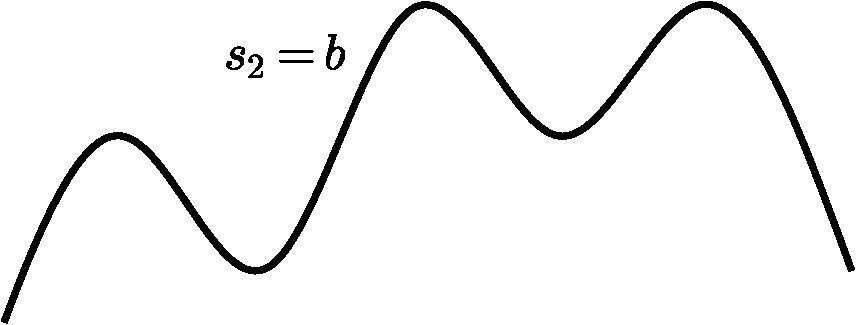
\includegraphics[width=0.26\textwidth]{figs/icefree.pdf}}

\pause
\smallskip
\item now \alert{margin overhang} is blocked:  \hfill \grey{\small real margins often fracture-dominated} \hspace{25mm}
\end{itemize}

\centerline{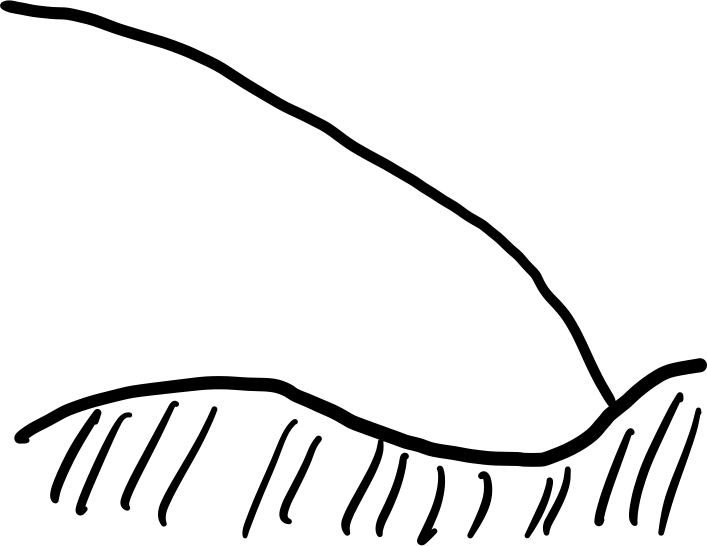
\includegraphics[height=16mm]{figs/wedge.png} \qquad 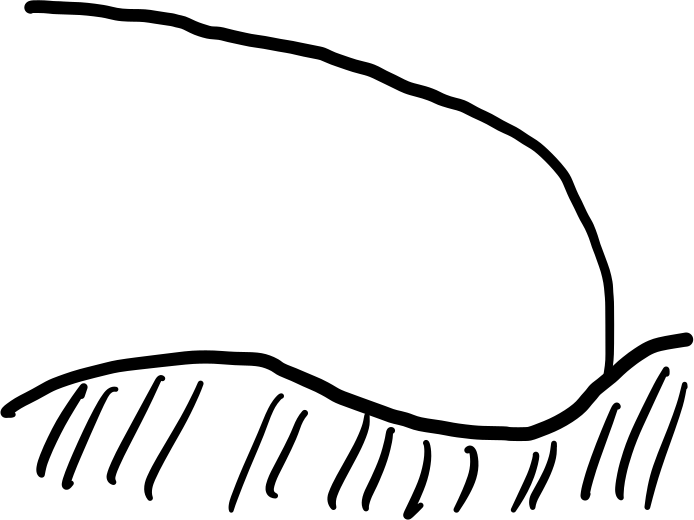
\includegraphics[height=16mm]{figs/unbounded.png} \hspace{15mm} 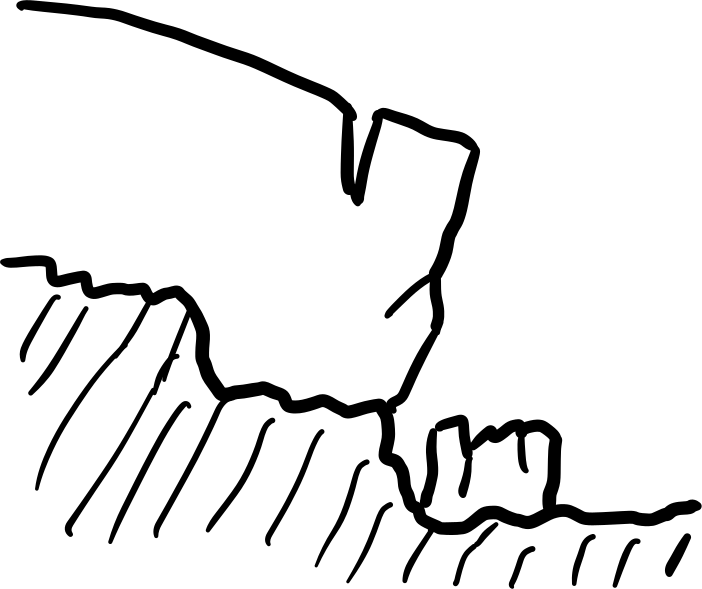
\includegraphics[height=17mm]{figs/realistic.png} \qquad 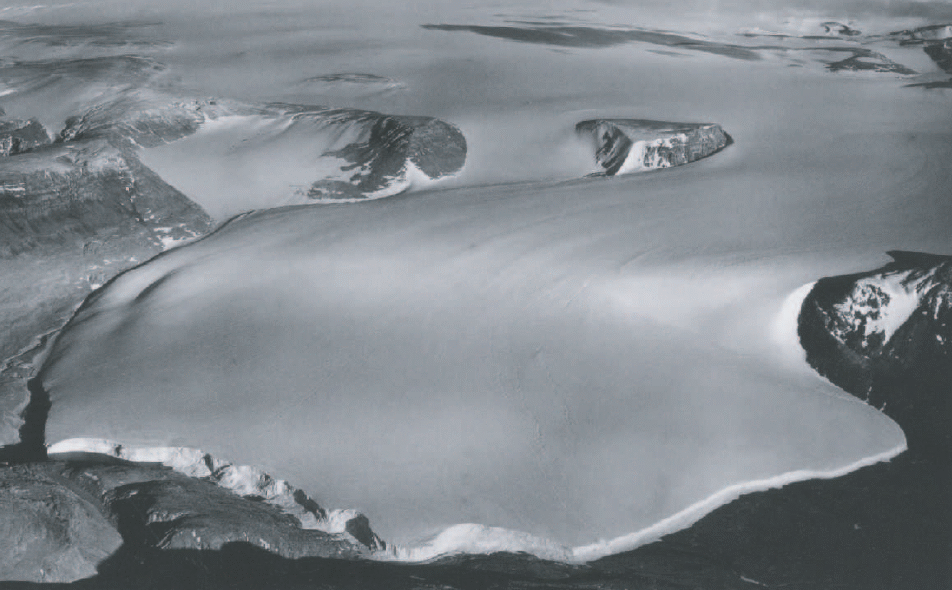
\includegraphics[height=19mm]{figs/polaris.png}}
\end{frame}


\begin{frame}{if surface-motion is coercive, then what?}

{\small
$$\Phi^\eps(s)[\omega] = -(1-\eps)\int_\Omega (\bu|_s \cdot \bn_s)\, \omega +\eps\,\gamma_0\eta_0^{5}\int_\Omega|\grad s|^{2}\grad s\cdot\grad\omega \qquad \text{with $\bu|_s$ from Stokes}$$

\begin{conjecture}[$4$-coercivity of regularized surface motion $\Phi^\eps$]
On $\cK = \{\sigma \ge b\} \subset \cX=W^{1,4}(\Omega)$, there exist $\eps>0$, $\eta_0>0$, and $\alpha>0$ so that $\Phi^\eps$ is $4$-coercive:
    $$\left(\Phi^\eps(\sigma)-\Phi^\eps(s)\right)[\sigma-s]\ge\alpha\|\sigma-s\|_\cX^4 \quad \text{for all } \sigma,s\in\cK.$$
\end{conjecture}
}

\smallskip
\begin{itemize}
\item suppose this conjecture is true?  then what?\footnote{B (2026), \href{https://arxiv.org/abs/2408.06470}{\emph{Surface elevation errors in FE Stokes models for glacier evolution}, arXiv:2408.06470}}

\pause
\smallskip
\item 2 important mathematical things follow:
   \begin{enumerate}
   \item for coupled surface-Stokes, the fully-implicit time-step problem is well-posed
   \item \emph{a priori} estimate exists for the surface elevation error in a finite element scheme
   \end{enumerate}
\item practical: get implicit Stokes schemes which are unconditionally-stable and capable of arbitrary retreat or advance during a time step
\end{itemize}
\end{frame}


\begin{frame}{$L^2$ evolution bound of Tominec et al (2026)}

\begin{itemize}
\item enter a different idea, a \alert{continuum stability bound for surface-Stokes}
\end{itemize}

\vspace{-3mm}
\begin{withpeople}{\vspace{3mm} \photo[8mm]{figs/people/itominec.jpg}{I.~Tominec} \photo[8mm]{figs/people/llundgren.jpg}{L.~Lundgren} \photo[8mm]{figs/people/alofgren.jpg}{A.~L\"ofgren} \photo[8mm]{figs/people/jahlkrona.png}{J.~Ahlkrona}}
\begin{theorem}[Tominec, Lundgren, L\"ofgren, Ahlkrona 2026]
Suppose $s(t,x)$ and $\bu(t,x,z)$ solve the time-dependent, coupled surface-Stokes problem, and write $\nu=\nu(D\bu)$ for the effective viscosity.  Then
  $$\frac{\rho g}{2}\frac{\partial}{\partial t}\|s\|_{L^2}^2 = -2\|\sqrt{\nu}\,D\bu\|_{L^2}^2+(\rho g a,s)_{L^2}.$$
It follows that: \quad $\|s\|_{L^2} \le \|s(t=0)\|_{L^2}+\int_0^t\|a\|_{L^2}$.

\smallskip
\grey{\small For the $D\bu$ integral the norm is $L^2(\Lambda(t); \RR^{3\times 3})$.  For the others it is $L^2(\Lambda(t)^\perp)$.}
\end{theorem}
\end{withpeople}

\smallskip
{\small
\noindent \textbf{proof.}  Test Stokes weak form with $\bu,p$, and weak surface equation with $s$. \hspace{12mm} $\qed$
}

\medskip
\begin{itemize}
\item idea: \, gravity-driven Stokes flow dissipates potential energy source $\rho g a$

\pause
\item however, $L^2$ norm bound on $s$ does not provide needed \alert{control of $\partial\Lambda(t)$ regularity for the Stokes problem}
\end{itemize}
\end{frame}


\section{state of play: explicit vs implicit}

\begin{frame}{performance modeling}

\begin{itemize}
\item B (2023): \, how to model solver efficiency?  \quad \alert{an update}
\pause
\item parameters:
    \begin{itemize}
    \item[$\lc$] $L$ typical domain length \hfill \pfcomm{for 2D domain $\Omega$}
    \item[$\lc$] $h$ resolution \hfill \pfcomm{for mesh over $\Omega$}
    \item[$\lc$] $m\sim L^2/h^2$ dofs $=$ number of nodes \hfill \pfcomm{for mesh over $\Omega$}
    \item[$\lc$] $U$ typical ice speed
    \item[$\lc$] $D$ typical diffusivity \hfill \pfcomm{from SIA formula}
    \item[$\lc$] $q$ number of time steps per model year needed for climate coupling
    \end{itemize}
\item cost in flops:

\vspace{-2mm}
\centerline{%
\hspace{30mm}
\begin{tabular}{ll}
Stokes solve                            & $O(m^{1+\alpha})$ \\
implicit SIA time-step solve            & $O(m^{1+\beta})$ \\
coupled implicit Stokes time-step solve & $O(m^{1+\gamma})$
\end{tabular}
}

\medskip
    \begin{itemize}
    \item[$\lc$] these are $m\to\infty$ asymptotic complexity models; note $\alpha,\beta,\gamma\ge 0$
    \end{itemize}

\item quantity of interest:

\vspace{-7mm}
\begin{align*}
\hspace{15mm} \text{\alert{FPMY}} &= \text{(flops per model year)} \\
  &= \text{(time steps per year)} \times \text{(flops per step)}
\end{align*}
\end{itemize}
\end{frame}


\newcommand{\sgrey}[1]{\grey{\small #1}}

\begin{frame}{performance modeling}

\begin{center}
\begin{tabular}{lllll}
\toprule
type & condition & dynamics & FPMY & \sgrey{examples} \\
\midrule
explicit & $\Delta t \le Ch^2/D$ & SIA & $O\left(D L^2\,h^{-4}\right)$ & \sgrey{mature ice sheet models} \\
         & $\Delta t \le Ch^2/D$ & Stokes & $O\left(D L^{2+2\alpha}\,h^{-(4+2\alpha)}\right)$ & \sgrey{current Stokes glacier models} \\
%         & $\Delta t \le Ch/U$   & Stokes & $O\left(U L^{2+2\alpha}\,h^{-(3+2\alpha)}\right)$ & \sgrey{\alert{TSSI}, Tominec et al (2026)} \\
         & $\Delta t \le Ch/U$   & Stokes & $O\left(U L^{2+2\alpha}\,h^{-(3+2\alpha)}\right)$ & \sgrey{Tominec et al (2026)} \\
implicit & $\Delta t \le 1/q$    & SIA & $O\left(q L^{2+2\beta}\,h^{-(2+2\beta)}\right)$ & \sgrey{B (2016); B \& Farrell (2024)} \\
         & $\Delta t \le 1/q$    & Stokes & $O\left(q L^{2+2\gamma}\,h^{-(2+2\gamma)}\right)$ & \sgrey{Ahlkrona, Henry, L\"ofgren (2026)} \\
\bottomrule
\end{tabular}
\end{center}

\begin{overprint}
\onslide<1>
\begin{itemize}
%\item TSSI (twice-stabilized semi-implicit scheme) avoids the $\Delta t=O(h^2)$ tragedy
\item Tominec et al (2026) scheme avoids the $\Delta t=O(h^2)$ tragedy
%\item warning: for implicit schemes solver complexity really matters!
%\item warning: for implicit schemes the constants in $O(\dots)$ are large
\end{itemize}
\onslide<2>
\begin{itemize}
\item if direct sparse linear algebra is used for explicit Stokes then $\alpha\approx 1$, at best
    \begin{itemize}
    \item[$\lc$] bad $O(h^{-5})$ scaling of FPMY \hfill \sgrey{makes it hard to do science}
    \end{itemize}
\item if solvers have mesh-dependent iterations then $\alpha,\beta,\gamma$ large
    \begin{itemize}
    \item[$\lc$] need multigrid
    \end{itemize}
\end{itemize}
\onslide<3>
\begin{itemize}
\item goal: \alert{$\gamma<0.5$ for implicit/coupled surface-Stokes}, giving better than $O(h^{-3})$ FPMY
\end{itemize}
\end{overprint}
\end{frame}


\setbeamertemplate{frame footer}{}

\begin{frame}{summary}

\begin{itemize}
\item \alert{surface-Stokes} is the canonical evolution model for glaciers:
    $$\text{surface kinematical equation} \, + \, \text{Stokes-type stress balance}$$
\item it's a free-boundary problem; glaciation is an output
    \begin{itemize}
    \item[$\lc$] as a dynamical system: \alert{differential-algebraic}, with \alert{inequality constraints}
    \end{itemize}
\item well-posed?
    \begin{itemize}
    \item[$\lc$] on bumpy beds, steady state is not unique
    \item[$\lc$] new $L^2$ stability bound (Tominec et al, 2026)
    \item[$\lc$] my conjecture: surface motion is coercive in $W^{1,4}$, if you regularize slightly
    \item[$\lc$] shallow approximation: various existence results (2002--2023)
    \end{itemize}
\item explicit vs implicit?
    \begin{itemize}
    %\item[$\lc$] twice-stabilized semi-implicit (Tominec et al, 2026) provably works well
    \item[$\lc$] mostly-explicit Tominec et al (2026) scheme a big improvement; provably works well
    \item[$\lc$] more-implicit schemes are under development \hfill \pfcomm{session CR2.8 at EGU?}
    \item[$\lc$] the \alert{scaling/complexity of solvers is important} \hfill \pfcomm{both Stokes and surface VI solvers}
    \end{itemize}
\end{itemize}

\centering
{\Large
\bigskip\bigskip
\alert{thank you for listening!}
}
\end{frame}


\appendix
\setbeamertemplate{page number in head/foot}{}

%\begin{frame}[allowframebreaks]{references}
\begin{frame}{references}
% inputed at end of talk4.tex

% blue link text; local, since talk4.tex inputs this inside a frame
\let\plainhref\href
\renewcommand{\href}[2]{\plainhref{#1}{\textcolor{icBlue}{#2}}}

\setlength{\leftmargini}{1em}  % bullets near the left margin, not indented
\begin{itemize}\setlength{\itemsep}{2pt}
\footnotesize
\item J.~Ahlkrona, A.~C.~J.~Henry, \& A.~L\"ofgren (2026). \href{https://doi.org/10.5194/gmd-19-2333-2026}{\emph{A fully implicit second order method for viscous free surface Stokes flow -- application to glacier simulations}}, Geosci.~Model Dev.~19, 2333--2348

%\item E.~Bueler (2016). \href{https://doi.org/10.1017/jog.2015.3}{\emph{Stable finite volume element schemes for the shallow ice approximation}}, J.~Glaciol.~62 (232), 230--242

\item E.~Bueler (2021). \href{https://doi.org/10.1137/20M135217X}{\emph{Conservation laws for free-boundary fluid layers}}, SIAM J.~Appl.~Math.~81 (5), 2007--2032

\item E.~Bueler (2023). \href{https://doi.org/10.1017/jog.2022.113}{\emph{Performance analysis of high-resolution ice-sheet simulations}}, J.~Glaciol.~69 (276), 930--935

\item E.~Bueler (2026). \href{https://arxiv.org/abs/2408.06470v3}{\emph{Surface elevation errors in finite element Stokes models for glacier evolution}}, preprint arXiv:2408.06470v3

%\item E.~Bueler \& P.~Farrell (2024). \href{https://doi.org/10.1137/23m1594200}{\emph{A full approximation scheme multilevel method for nonlinear variational inequalities}}, SIAM J.~Sci.~Comput.~46 (4), A2421--A2444

\item N.~Calvo, J.~D\'iaz, J.~Durany, E.~Schiavi, \& C.~V\'azquez (2002). \href{https://doi.org/10.1137/S0036139901385345}{\emph{On a doubly nonlinear parabolic obstacle problem modelling ice sheet dynamics}}, SIAM J.~Appl.~Math.~63 (2), 683--707

%\item R.~Falk (1974). \href{https://doi.org/10.1090/S0025-5718-1974-0391502-8}{\emph{Error estimates for the approximation of a class of variational inequalities}}, Math.~Comp.~28 (128), 963--971

\item G.~Jouvet \& E.~Bueler (2012). \href{https://doi.org/10.1137/110856654}{\emph{Steady, shallow ice sheets as obstacle problems: well-posedness and finite element approximation}}, SIAM J.~Appl.~Math.~72 (4), 1292--1314

\item G.~Jouvet \& J.~Rappaz (2011). \href{https://doi.org/10.1155/2011/164581}{\emph{Analysis and finite element approximation of a nonlinear stationary Stokes problem arising in glaciology}}, Adv.~Numer.~Anal.~2011, 164581

%\item D.~Kinderlehrer \& G.~Stampacchia (1980). \emph{An Introduction to Variational Inequalities and their Applications}, Academic Press

%\item A.~L\"ofgren, J.~Ahlkrona, \& C.~Helanow (2022). \href{https://doi.org/10.1016/j.jcpx.2022.100114}{\emph{Increasing stable time-step sizes of the free-surface problem arising in ice-sheet simulations}}, J.~Comput.~Phys.:~X 16, 100114

\item P.~Piersanti \& R.~Temam (2023). \href{https://doi.org/10.1515/anona-2022-0280}{\emph{On the dynamics of grounded shallow ice sheets: modeling and analysis}}, Adv.~Nonlinear Anal.~12, 20220280

\item I.~Tominec, L.~Lundgren, A.~L\"ofgren, \& J.~Ahlkrona (2026). \href{https://doi.org/10.1093/imanum/drag117}{\emph{Free-surface Stokes problem: stability estimates and time-step improvements}}, IMA J.~Numer.~Anal.
\end{itemize}

\end{frame}


\begin{frame}[standout]
extra slides
\end{frame}


\begin{frame}{a mostly-explicit solver that works}

\begin{itemize}
\item from Josefin Ahlkrona's group (L\"ofgren et al 2022, Tominec et al 2026)
\end{itemize}

{\small
\begin{block}{twice-stabilized semi-implicit (TSSI) scheme for surface-Stokes}
\begin{enumerate}
\item At $t_k$, solve weak Stokes for $\bu,p$ on current geometry, with symmetrized \alert{load stabilization}:
    $$\int_{\Lambda^k}2\nu\,D\bu:D\bv-p\Div\bv-q\Div\bu-\rho\bg\cdot\bv+\alert{\int_{\Gamma_s^k}\rho g\Delta t\left[\tfrac{1}{2}\bu\cdot\bn_{s^k}+a\right]\bv\cdot\hat\bn}=0 \qquad \forall \bv,q$$
\item Choose $\Delta t=C_{\text{CFL}}\min h/|\bu|$, then update surface as a VI for $s^{k+1}\in\cK_h=\{\sigma\,:\,\sigma\ge b_h\}$, with implicit \alert{edge stabilization}, $J_k(s,r)=\sum_e\int_e\tfrac{1}{2}h_e^2\big|\bu|_{s^k}\big|\jump{\grad s}\jump{\grad r}\,dS$:
    $$\int_\Omega\left(\frac{s^{k+1}-s^k}{\Delta t}-\bu|_{s^k}\cdot\bn_{s^k}-a\right)(\sigma-s^{k+1})+\alert{J_k\left(s^{k+1},\sigma-s^{k+1}\right)}\ge 0 \qquad \forall \sigma\in\cK_h$$
\item Repeat.
\end{enumerate}
\end{block}
}

\begin{itemize}
\item one Stokes solve per step
\item one (cheap!) variational inequality (VI) solve per step
\end{itemize}
\end{frame}


\begin{frame}{a mostly-explicit solver that is provably stable}

\begin{theorem}[Tominec et al 2026]
In TSSI scheme, the new solution is bounded by the data:
    $$\|s^{k+1}\|_{L^2}^2+\frac{4\Delta t}{\rho g}\|\sqrt{\mu}D\bu\|_{L^2}^2+2\Delta t\,J_k(s^{k+1},s^{k+1})\le\|s^k+\Delta t \,a\|_{L^2}^2.$$
\end{theorem}

\medskip
\begin{itemize}
\item \alert{arbitrary time steps are stable}
\item TSSI is consistent, and globally mass-conserving
\item CFL is still needed for accurate moving margins
    \begin{itemize}
    \item[$\lc$] the velocity is explicit, so margin can advance at most one element per step
    \end{itemize}
\end{itemize}
\end{frame}

\end{document}
